\documentclass[a4paper]{report}
\usepackage[utf8]{inputenc}
\usepackage[T1]{fontenc}
\usepackage{textcomp}

\usepackage{url}

% \usepackage{hyperref}
% \hypersetup{
%     colorlinks,
%     linkcolor={black},
%     citecolor={black},
%     urlcolor={blue!80!black}
% }

\usepackage{graphicx}
\usepackage{float}
\usepackage[usenames,dvipsnames]{xcolor}

% \usepackage{cmbright}

\usepackage{amsmath, amsfonts, mathtools, amsthm, amssymb}
\usepackage{mathrsfs}
\usepackage{cancel}

\newcommand\N{\ensuremath{\mathbb{N}}}
\newcommand\R{\ensuremath{\mathbb{R}}}
\newcommand\F{\ensuremath{\mathscr{F}}}
\newcommand\Z{\ensuremath{\mathbb{Z}}}
\renewcommand\O{\ensuremath{\emptyset}}
\newcommand\Q{\ensuremath{\mathbb{Q}}}
\newcommand\C{\ensuremath{\mathbb{C}}}
\let\implies\Rightarrow
\let\impliedby\Leftarrow
\let\iff\Leftrightarrow
\let\epsilon\varepsilon

% horizontal rule
\newcommand\hr{
    \noindent\rule[0.5ex]{\linewidth}{0.5pt}
}

\usepackage{tikz}
\usepackage{tikz-cd}

% theorems
\usepackage{thmtools}
\usepackage[framemethod=TikZ]{mdframed}
\mdfsetup{skipabove=1em,skipbelow=0em, innertopmargin=5pt, innerbottommargin=6pt}

\theoremstyle{definition}

\makeatletter

\declaretheoremstyle[headfont=\bfseries\sffamily, bodyfont=\normalfont, mdframed={ nobreak } ]{thmgreenbox}
\declaretheoremstyle[headfont=\bfseries\sffamily, bodyfont=\normalfont, mdframed={ nobreak } ]{thmredbox}
\declaretheoremstyle[headfont=\bfseries\sffamily, bodyfont=\normalfont]{thmbluebox}
\declaretheoremstyle[headfont=\bfseries\sffamily, bodyfont=\normalfont]{thmblueline}
\declaretheoremstyle[headfont=\bfseries\sffamily, bodyfont=\normalfont, numbered=no, mdframed={ rightline=false, topline=false, bottomline=false, }, qed=\qedsymbol ]{thmproofbox}
\declaretheoremstyle[headfont=\bfseries\sffamily, bodyfont=\normalfont, numbered=no, mdframed={ nobreak, rightline=false, topline=false, bottomline=false } ]{thmexplanationbox}


\declaretheorem[numberwithin=chapter, style=thmgreenbox, name=Definition]{definition}
\declaretheorem[sibling=definition, style=thmredbox, name=Corollary]{corollary}
\declaretheorem[sibling=definition, style=thmredbox, name=Proposition]{prop}
\declaretheorem[sibling=definition, style=thmredbox, name=Theorem]{theorem}
\declaretheorem[sibling=definition, style=thmredbox, name=Lemma]{lemma}



\declaretheorem[numbered=no, style=thmexplanationbox, name=Proof]{explanation}
\declaretheorem[numbered=no, style=thmproofbox, name=Proof]{replacementproof}
\declaretheorem[style=thmbluebox,  numbered=no, name=Exercise]{ex}
\declaretheorem[style=thmbluebox,  numbered=no, name=Example]{eg}
\declaretheorem[style=thmblueline, numbered=no, name=Remark]{remark}
\declaretheorem[style=thmblueline, numbered=no, name=Note]{note}

\renewenvironment{proof}[1][\proofname]{\begin{replacementproof}}{\end{replacementproof}}

\AtEndEnvironment{eg}{\null\hfill$\diamond$}%

\newtheorem*{uovt}{UOVT}
\newtheorem*{notation}{Notation}
\newtheorem*{previouslyseen}{As previously seen}
\newtheorem*{problem}{Problem}
\newtheorem*{observe}{Observe}
\newtheorem*{property}{Property}
\newtheorem*{intuition}{Intuition}


\usepackage{etoolbox}
\AtEndEnvironment{vb}{\null\hfill$\diamond$}%
\AtEndEnvironment{intermezzo}{\null\hfill$\diamond$}%




% http://tex.stackexchange.com/questions/22119/how-can-i-change-the-spacing-before-theorems-with-amsthm
% \def\thm@space@setup{%
%   \thm@preskip=\parskip \thm@postskip=0pt
% }

\usepackage{xifthen}

\def\testdateparts#1{\dateparts#1\relax}
\def\dateparts#1 #2 #3 #4 #5\relax{
    \marginpar{\small\textsf{\mbox{#1 #2 #3 #5}}}
}

\def\@lesson{}%
\newcommand{\lesson}[3]{
    \ifthenelse{\isempty{#3}}{%
        \def\@lesson{Lecture #1}%
    }{%
        \def\@lesson{Lecture #1: #3}%
    }%
    \subsection*{\@lesson}
    \testdateparts{#2}
}

% fancy headers
\usepackage{fancyhdr}
\pagestyle{fancy}

% \fancyhead[LE,RO]{Gilles Castel}
\fancyhead[RO,LE]{\@lesson}
\fancyhead[RE,LO]{}
\fancyfoot[LE,RO]{\thepage}
\fancyfoot[C]{\leftmark}
\renewcommand{\headrulewidth}{0pt}

\makeatother

% figure support (https://castel.dev/post/lecture-notes-2)
\usepackage{import}
\usepackage{xifthen}
\pdfminorversion=7
\usepackage{pdfpages}
\usepackage{transparent}
\newcommand{\incfig}[1]{%
    \def\svgwidth{\columnwidth}
    \import{./figures/}{#1.pdf_tex}
}

% %http://tex.stackexchange.com/questions/76273/multiple-pdfs-with-page-group-included-in-a-single-page-warning
\pdfsuppresswarningpagegroup=1

\author{Aamod Varma}
\setlength{\parindent}{0pt}


\title{Intro to Proofs: HW06}
\author{Aamod Varma}
\graphicspath{ {./} }
\begin{document}
\maketitle
\date{}
    
\subsection*{11.1.1}
    
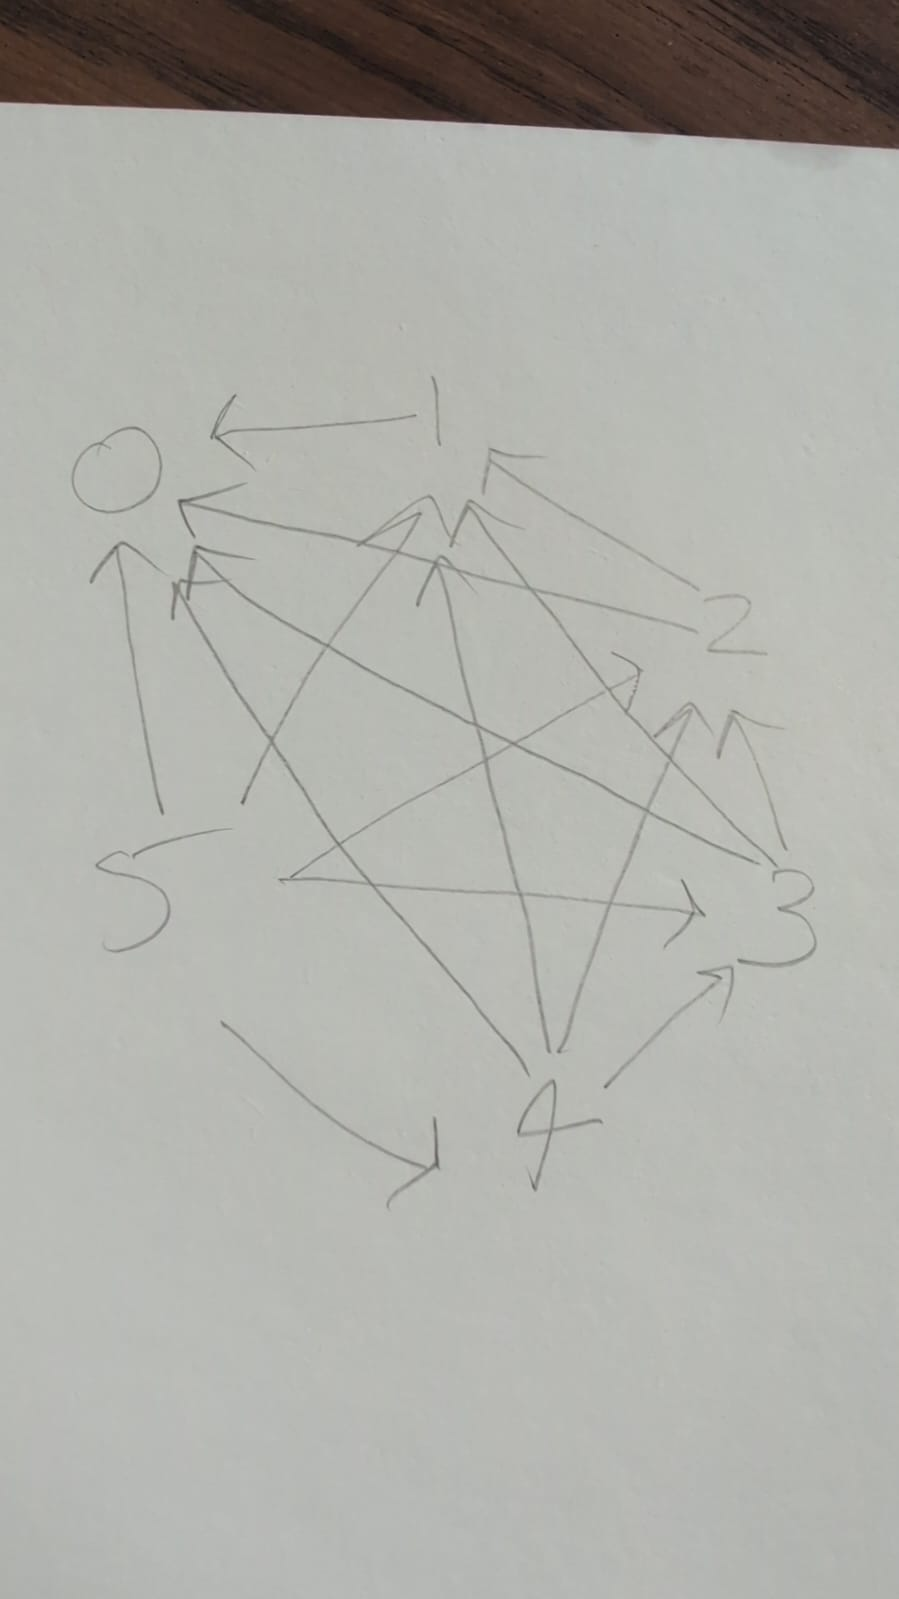
\includegraphics[scale=.2]{Untitled}

\subsection*{11.1.4}
$A = \{0,1,2,3,4,5\}$ and  $$R = \{(0,0),(1,1),(2,2),(3,3),(4,4),(5,5),(0,4),(4,0),(1,3),(3,1),(1,5),(5,1),(2,4),(4,2)\}$$

\subsection*{11.1.11}
Consider $|A| = n$ then the number of pairs of elements  $(a,b)$  where $a,b \in A$ is $n^2$. Now a relation can be defined as containing any possible combination of this set. So the set of relations would be the power set of the set of the pairs which would be $$2^{n^2}$$

\subsection*{11.2.4}
1. Reflexivity

For reflexivity we need $\forall a \in A, aRa$. We see that $aRa, bRb, cRc, dRd$ therefore $A$is reflexive.

2. Symmetric

We need for any  $aRb \implies bRa$. We see this is true by observation. For any pair  $(x,y)$ we see that $(y,x)$ is in R as well. So it is symmetric.


3. Transitivity

We need $aRb, bRc \implies aRc$. We see that this is also true for any pair of relations in our form. So it is transitive.

Also notice that $R$ contains all possible pairs of elements of $A$.

\subsection*{11.2.5}
1. Reflexive


For reflexivity we need $\forall x \in \R, xRx$. However in our relation thish is only true for two values $0,\sqrt{2}$. Hence it is not reflexive. So for instance, $(1,1) \not \in R$ but  $1 \in \R$.

2. Symmetric

We see that for any $aRb$, $bRa$ is true. This is automatically true for $(0,0)$ and $(\sqrt 2, \sqrt 2)$ as they are symmetric. We see for $(0,\sqrt 2)$ that $(\sqrt 2,0)$ is also in $R$ same can be said for $(\sqrt 2, 0)$. So it is symmetric.

3. Transivity

We see that for any $aRb, bRc$  that $aRc$ is true. So it is transitive. 


\subsection*{11.2.6}
We have $R = \{(x,x): x \in \Z\}$

1. Reflexive.

We see that  $\forall x \in \X$, $(x,x) \in R$ by definition. So it is reflexive.

2. Symmetric

As our relation only contains pairs of $(x,x)$ it is automatically symmetric as interchanging the numbers gives us the same pair. So it is symmetric.

3. Transitive

For transitivity we need, $aRb, bRc \implies aRc$. However in ours list $a = b$ by definition and $b = c$ by definition hence $a= c \implies aRc$. Hence it is transitive.

\subsection*{11.2.13}
We have $R = \{(x,y) \in \R \times  \R : x - y  \in \Z\}$

1. Reflexive

We need to show that $\forall x \in R$, $xRx$. 

Take any  $x \in R$ we have $x - x = 0 \in Z$. Hence $x$ is  related to itself or $xRx$ is true. So it is reflexive.

2. Symmetric

For any $xRy$ we need to show  $yRx$.

Take a given  $xRy$ this implies that $x - y \in \Z$ so  $x - y = k$ such that  $k \in Z$. Now multiplying  $-1$ on both sides we get, $y - x = -k$. If  $ k \in Z $ then $ -k \in Z$ so $y -x \in \Z$ which means that $yRx$.

Therefore  $R$ is symmetric.

3. Transitive

We need to show $aRb, bRc \implies aRc$. $aRb$ means $a - b \in \Z$ or $a - b = k_1$. Similarly, $b - c = k_2$.

Now add the two equation we get, $a - b + b - c = k_1 + k_2$ or $a - c = k_1 + k_2 \in \Z$. 

Therefore $aRc$ is true. Hence $R$ is transitive.


\subsection*{11.2.14}

\begin{proof}
We are given that $R$ is symmetric and transitive. We also know that $\exists a \in A$ such that $aRx, \forall x \in A$.

Now because it is symetric we know that $aRx \implies xRa$. So we have $aRx, xRa$ is true.

If it is symmetric then $aRb, bRc \implies aRc$. So $xRa, aRx \implies xRx$  where $x$ is any element of $A$.

Se showed that $\forall x \in A, xRx$ is true. Hence it is reflexive.

\end{proof}
\subsection*{11.2.15}
\begin{proof}
    We disprove by counterexample. Consider $A = \{0,1\}$

    The relation,  
    $$ R = \{(0,0)\} $$ is symmetriic because $(0,0) \in R \implies (0,0) \in R$ and transitive. Howeer it is not reflexive as $(1,1) \not \in R$.
\end{proof}


\subsection*{11.2.18}
For $>$ we have, Reflexive: no, Symmetric: no, Transitive: yes. And for $\ge$ we have, Reflexive: yes, Symmetric: no, Transitive: yes.



\subsection*{11.3.3}

We have $A = \{a,b,c,d,e\}$ and  $R$ has three equivalence classes. It is also given that $(a,d),(b,c) \in R$

Let the three equivalence classes be, $\{a,d\}, \{b,c\}, \{e\}$ 

So the equivalence relation defined using these classes would be, 
$$ R = \{(a,a), (b,b), (c,c), (d,d), (e,e), (a,d), (d,a), (b,c), (c,b)\} $$ 

We see that $R$ is an equivalence relation because it is reflexive symmetric and transitive.


\subsection*{11.3.6}
Given $A = \{a,b,c\}$. The differenr equivalence relation on $A$ will currespond to the different equivalence classes in $A$. These are, 

$$ \{a\}, \{b\}, \{c\} \text{ where R } = \{(a,a),(b,b),(c,c)\}$$ 
$$ \{c\}, \{a,b\}\text{ where R } = \{(a,a),(b,b),(c,c),(a,b),(b,a)\}$$ 
$$ \{a\},\{b,c\}\text{ where R } = \{(a,a),(b,b),(c,c), (b,c),(c,b)\}$$ 
$$  \{b\},\{a,c\}\text{ where R } = \{(a,a),(b,b),(c,c),(a,c),(c,a)\}$$ 
$$ \{a,b,c\}\text{ where R } = \{(a,a),(b,b),(c,c),(a,b),(b,a),(a,c),(c,a),(b,c),(c,b)\}$$ 


\subsection*{11.3.9}
We have a relation $R$ on $\Z$ such that 
$$ xRy \text{ iff } 4 | (x + 3y)$$ 

First we see reflexivity, we need $xRx$. We see that for any $x \in \Z$, 
$$ x + 3y = x + 3x = 4x \implies 4 | (x + 3x) \implies xRx $$ 
So, $R$ is reflexive.

Now for it to be symmetric we need $xRy \implies yRx$. Assuem $xRy$ is true for some $x,y \in \Z$. We have, 
$$ xRy \implies  x + 3y = 4k $$ 

Now, $$y + 3x = y + 3(4k - 3y) = y + 12k - 9y = 12k - 8y = 4(3k - 2y) = 4k_0 \implies yRx$$

So, $R$ is symmetric

For transitivity we need, $xRy, yRz \implies xRz$. 
$$ xRy  \implies x + 3y = 4k_1 \text{ and } yRz \implies y + 3z = 4k_2$$ 
$$  x + 3y + y + 3z = 4(k_1 + k_2)$$ 
$$ x + 3z  = 4(k_1 +k_2 - y) = 4k_3 \implies xRz $$ 

So $R$ is transitive.


The equivalnece classes of R would be, 
$$ [0] =  xR0 = \{4 | x + 0:x \in \Z\} = \{\dots, -8,-4,0,4,8,\dots\} $$ 
$$ [1] =  xR1 = \{4 | x + 3:x \in \Z\} = \{\dots,-7, -3, 1, 5, 9,\dots\} $$ 
$$ [2] =  xR2 = \{4 | x + 6 = 4 | x + 2:x \in \Z\} = \{\dots-6,-2,2,6,10,\dots\} $$ 
$$ [3] =  xR3 = \{4 | x + 9 = 4 | x + 1:x \in \Z\} = \{\dots-1,,3,7,11,15,\dots\} $$ 


\subsection*{11.3.12}

Take $A = (a,b,c)$. Let our two relations currespond to the equivalence classes as follows,  
$$ \{a,b\},\{c\} \text{ so } R_1= \{(a,a),(b,b),(c,c),(a,b),(b,a)\}$$ 
$$ \{a\},\{b,c\} \text{ so } R_2=  \{(a,a),(b,b),(c,c),(b,c),(c,b)\}$$ 


And we have, 
$$ R_3 = R_1\cup R_2 = \{(a,a),(b,b),(c,c),(a,b),(b,a), (b,c), (c,b)\} $$ 

We see that in this union transitivity does not hold as  $(a,b) \in R_3$ and $(b,c) \in R_3$ but $(a,c) \not \in R_3$. 

Hence we disprove by counterexample


\subsection*{11.4.2}
All the parittions are as follows, 

$$ \{a\}, \{b\},\{c\} $$ 
$$ \{a,b\},\{c\} $$ 
$$ \{a,c\},\{b\} $$ 
$$ \{b,c\},\{a\} $$ 
$$ \{b,c,a\} $$ 






\subsection*{11.4.6}
The currensponding equivalcne relation would be, 
$$R =  \{(0,0), (-1,-1), (1,1), (-1,1), (1,-1), \dots, (-k,-k), (k,k), (-k, k), (k, -k)\} $$
For any $k \in \Z$




 















\end{document}

